\documentclass[unknownkeysallowed,xcolor=table]{beamer}
 
\usepackage [T2A,T1] {fontenc}
\usepackage[utf8]{inputenc}
\usepackage[english,russian]{babel}
\usepackage{amsmath}
\usepackage{listings}
\usepackage{url}
\usepackage{textcomp}
\usepackage{multirow}

\setbeamertemplate{navigation symbols}{}

\newcommand{\textapprox}{\raisebox{0.5ex}{\texttildelow}}

\lstnewenvironment{cmdline}
  {\lstset{basicstyle=\ttfamily\scriptsize,keywordstyle=\color{blue},
           language={bash}}}
  {}
  
\lstnewenvironment{cmdlinelarge}
  {\lstset{basicstyle=\ttfamily\small,keywordstyle=\color{blue},
           language={bash}}}
  {}
  
\colorlet{mygreen}{green!60!blue}
\colorlet{mymauve}{red!60!blue}
\definecolor{pblue}{rgb}{0.1, 0.2, 0.8}

\newcommand{\rarr}{$\rightarrow$}

\lstset{
      basicstyle=\ttfamily\small,
      commentstyle=\color{mygreen},
      keywordstyle=\color{blue},
      numberstyle=\tiny\color{blue},
      stringstyle=\color{mymauve},
      columns=fullflexible,
      breaklines=true,
      postbreak=\mbox{\textcolor{red}{\ensuremath{\hookrightarrow}\space}},
      literate={~} {\textapprox}{1},
      language={[11]C++}
}

\makeatletter
\newcommand{\srcmediumsize}{\@setfontsize{\srcmediumsize}{7pt}{7pt}}
\makeatother

\makeatletter
\newcommand{\srcbigsize}{\@setfontsize{\srcbigsize}{8pt}{8pt}}
\makeatother

\makeatletter
\newcommand{\srcsize}{\@setfontsize{\srcsize}{6pt}{6pt}}
\makeatother

\makeatletter
\newcommand{\srcsmallsize}{\@setfontsize{\srcsmallsize}{5pt}{5pt}}
\makeatother

\newcommand{\rot}[1]{\makebox[1em][l]{\rotatebox{45}{#1}}}

\title[C++]
{Программирование на языке C++}
 
\subtitle{Вводный курс}
 
\author[А.~Б.~Морозов]
{
  \texorpdfstring{Александр Морозов\newline\href{mailto:gelu.speculum@gmail.com}{gelu.speculum@gmail.com}}
  {Александр Морозов}
}
  
\date[ITMO 2020]
{ИТМО, весенний семестр 2020}
 
\logo{%
  \makebox[0.97\paperwidth]{%
    
\includegraphics[align=c,width=2cm,keepaspectratio]{itmo_logo.png}
    \hfill
    
\includegraphics[align=c,width=1.5cm,keepaspectratio]{itiviti_logo.png}
  }
}

\AtBeginSection[]
{
  \begin{frame}
    \frametitle{Содержание}
    \tableofcontents[currentsection]
  \end{frame}
}

\begin{document}

\frame{\titlepage}

%-------------------------------------------------

\section{Коллекции}

\begin{frame}{Коллекции}

Коллекция -- набор объектов одного типа (элементов), допускающий как операции со всей коллекцией в целом, так и с отдельными элементами. \\
Другое название -- контейнер.

\vspace{2em}

Экземпляр коллекции хранит элементы внутри себя, копирование или перемещение экземпляра коллекции приводит к копированию или перемещению всех её элементов.

\end{frame}

\begin{frame}{Некоторые свойства коллекций}

Общие:

\vspace{0.5em}

\begin{itemize}
  \item хранение множества элементов одного типа \vspace{0.5em}
  \item последовательный доступ ко всем элементам \vspace{0.5em}
  \item операции над элементами: немодифицирующий доступ (чтение), модифицирующий доступ (запись), удаление и добавление
\end{itemize}

\vspace{1em}

Различающиеся:

\vspace{0.5em}

\begin{itemize}
  \item эффективность реализации тех или иных операций \vspace{0.5em}
  \item доступ к элементам в определенном порядке \vspace{0.5em}
  \item некоторые специфические операции
\end{itemize}

\end{frame}

\begin{frame}{Понятие вычислительной сложности}

\begin{itemize}
  \item вычислительные затраты на обработку \vspace{0.5em}
  \item затраты памяти на представление или обработку
\end{itemize}

\vspace{1em}

\begin{center}
$f(n) \in O(g(N))$
\end{center}

\vspace{0.5em}

\begin{itemize}
  \item $O(1)$
  \item $O(log(N))$
  \item $O(N)$
  \item $O(N^2)$
  \item $O(2^N)$
  \item $O(N!)$
\end{itemize}

\end{frame}

\begin{frame}[fragile]{Стандартные коллекции: простые последовательности}

\begin{itemize}
  \item \lstinline{std::array} -- массив элементов со статическим размером \vspace{0.7em}
  \item \lstinline{std::vector} -- массив элементов с динамическим размером \vspace{0.7em}
  \item \lstinline{std::deque} -- двусторонняя очередь \vspace{0.7em}
  \item \lstinline{std::forward_list} -- односвязный список \vspace{0.7em}
  \item \lstinline{std::list} -- двусвязный список
\end{itemize}

\end{frame}

\begin{frame}[fragile]{Стандартные коллекции: упорядоченные множества}

\begin{itemize}
  \item \lstinline{std::set} -- упорядоченное множество \vspace{0.7em}
  \item \lstinline{std::map} -- упорядоченный ассоциативный массив \vspace{0.7em}
  \item \lstinline{std::multiset} -- упорядоченное мультимножество \vspace{0.7em}
  \item \lstinline{std::multimap} -- упорядоченный ассоциативный массив с повторением ключей
\end{itemize}

\end{frame}

\begin{frame}[fragile]{Стандартные коллекции: неупорядоченные множества}

\begin{itemize}
  \item \lstinline{std::unordered_set} -- неупорядоченное множество \vspace{0.7em}
  \item \lstinline{std::unordered_map} -- неупорядоченный ассоциативный массив \vspace{0.7em}
  \item \lstinline{std::unordered_multiset} -- неупорядоченное мультимножество \vspace{0.7em}
  \item \lstinline{std::unordered_multimap} -- неупорядоченный ассоциативный массив с повторением ключей
\end{itemize}

\end{frame}

\begin{frame}[fragile]{Адаптеры коллекций}

\begin{itemize}
  \item \lstinline{std::stack} -- LIFO \vspace{0.7em}
  \item \lstinline{std::queue} -- FIFO \vspace{0.7em}
  \item \lstinline{std::priority_queue} -- приоритетная очередь, быстрый доступ к наибольшему элементу
\end{itemize}

\end{frame}

\begin{frame}{Внутреннее представление}

\begin{itemize}
  \item непрерывная область памяти -- \lstinline{std::array}, \lstinline{std::vector} \vspace{1em}
  \item набор независимых подобластей -- \lstinline{std::deque} \vspace{1em}
  \item каждый элемент в отдельном узле списка -- \lstinline{std::forward_list}, \lstinline{std::list} \vspace{1em}
  \item дерево -- \lstinline{std::set}, \lstinline{std::map}, \lstinline{std::multiset}, \lstinline{std::multimap} \vspace{1em}
  \item хеш-массив -- \lstinline{std::unordered_set}, \lstinline{std::unordered_map}, \lstinline{std::unordered_multiset}, \lstinline{std::unordered_multimap}
\end{itemize}

\end{frame}

\begin{frame}[fragile]{Сложность некоторых операций}

\begin{center}
\begin{tabular}{ l | c c c c c }
  \hline
    & \rot{vector} & \rot{deque} & \rot{list} & \rot{map} & \rot{unordered\_map} \\
  \hline
    fill & $O(N)$ & $O(N)$ & $O(N)$ & $O(N \cdot log(N))$ & $O(N)$ \\
    add & $O(N)$ & $O(1)$ & $O(1)$ & $O(log(N))$ & $O(1)$/$O(N)$ \\
    insert & $O(N)$ & $O(N)$ & $O(1)$ & $O(log(N))$ & $O(1)$/$O(N)$ \\
    at & $O(1)$ & $O(1)$ & $O(N)$ & $O(log(N))$ & $O(1)$/$O(N)$ \\
\end{tabular}
\end{center}

\end{frame}

%-------------------------------------------------

\section{Итераторы}

\begin{frame}{Итераторы}

Итератор -- абстракция ``указателя'' на элемент некоторой последовательности.

\vspace{2em}

Тип итератора может быть связан с конкретным типом коллекции/контейнера, но бывают и иные итераторы. Реализация скрывает в себе подробности доступа к указываемому элементу коллекции и связь с ``соседними'' элементами.

\vspace{2em}

Каждая коллекция задает некоторый порядок на множестве элементов, если представить это как массив в памяти, итераторы имитируют указатели на элементы этого массива.

\end{frame}

\begin{frame}[fragile]{Итераторы и указатели: сходство}

\begin{itemize}
  \item Разыменование для доступа к элементу (операторы \lstinline{*} и \lstinline{->})
  \item Равенство/неравенство
  \item Инкремент для смещения к следующему элементу
  \item Итератор может указывать на ``после последнего элемента'' коллекции
  \item Некоторые итераторы можно декрементировать для смещения к предыдущему элементу
  \item Над некоторыми итераторами возможна арифметика, как с указателями
  \item Некоторые итераторы поддерживают доступ по индексу (аналогично указателям)
  \item Некоторые итераторы можно сравнивать \lstinline{<}/\lstinline{>}
\end{itemize}

\end{frame}

\begin{frame}{Итераторы и указатели: различия}

Указатель удовлетворяет ``концепции итератора'', но итераторы коллекций от указателей отличаются.

\vspace{1em}

\begin{itemize}
  \item Является сложным типом (классом)
  \item Эффективность операций зависит от конкретной реализации
  \item Всегда связан с конкретным объектом коллекции или иной сущности
  \item Некоторые действия над объектом коллекции могут инвалидировать итератор
  \item Для итераторов не работает приведение типов, возможное для указателей
\end{itemize}

\end{frame}

\begin{frame}[fragile]{Концепция: итератор}

\begin{itemize}
  \item Объект можно копировать \vspace{1em}
  \item Определен оператор \lstinline{*} \vspace{1em}
  \item Определен оператор префиксного инкремента (условие -- итератор должен быть указывать на элемент коллекции; результатом будет либо итератор, указывающий на следующий элемент, либо на после последнего)
\end{itemize}

\end{frame}

\begin{frame}[fragile]{Концепция: итератор на чтение (input)}

\begin{itemize}
  \item Удовлетворяет требованиям итератора \vspace{0.7em}
  \item Объекты можно сравнивать на равенство/неравенство \vspace{0.7em}
  \item Определен оператор \lstinline{->} \vspace{0.7em}
  \item Определен оператор постфиксного инкремента \vspace{0.7em}
  \item Не гарантирована валидность копий итератора после его инкремента
\end{itemize}

\vspace{1em}

Таким образом, не гарантирована возможность многократного прохода по элементам, только однократного.

\end{frame}

\begin{frame}[fragile]{Концепция: итератор на запись (output)}

\begin{itemize}
  \item Удовлетворяет требованиям итератора
  \item Определен оператор постфиксного инкремента
  \item Валидно выражение \lstinline{*i = x} где \lstinline{i} -- объект итератора, а \lstinline{o} некоторое значение; после выполнения этого выражение не гарантируется разыменуемость итератора или валидность его предыдущих копий
  \item Не гарантирована валидность копий итератора после его инкремента
  \item Операцию разыменования допустимо использовать только для присвоения значения
\end{itemize}

\vspace{1em}

Таким образом, не гарантирована возможность многократного прохода по элементам, только однократного.

\end{frame}

\begin{frame}[fragile]{Концепция: мутабельный итератор (input and output)}

Если итератор удовлетворяет обоим концепциям -- input и output, то его называют mutable, это значит, что указываемые значения можно читать, а можно присваивать им другие значения.

\end{frame}

\begin{frame}[fragile]{Концепция: итератор непрерывной области (contiguous)}

\begin{itemize}
  \item Удовлетворяет требованиям итератора \vspace{1em}
  \item Элементы коллекции, с которой связан итератор, размещены в непрерывной области в памяти и в том порядке, в котором осуществляется обход с помощью итераторов \vspace{1em}
  \item Валидна операция \lstinline{*(a + n)} и эквивалентна \lstinline{*(&(*a) + n)}
\end{itemize}

\end{frame}

\begin{frame}[fragile]{Концепция: итератор прямого обхода (forward)}

\begin{itemize}
  \item Удовлетворяет требованиям итератора на чтение
  \item \lstinline{a == b} $\Leftrightarrow$ \lstinline{&(*a) == &(*b)} (либо оба не разыменуются)
  \item Инкремент итератора не меняет валидность его копий
  \item Инкремент итератора не меняет результат разыменования его копий
  \item Равенство итераторов гарантирует равенство результатов их инкремента
  \item Если итератор является мутабельным, то присвоение через итератор не меняет его валидность или валидность его копий
\end{itemize}

\vspace{1em}

Таким образом, гарантирована возможность многократного прохода по элементам.

\end{frame}

\begin{frame}[fragile]{Концепция: итератор двустороннего обхода (bidirectional)}

\begin{itemize}
  \item Удовлетворяет требованиям итератора прямого обхода \vspace{1em}
  \item Определен оператор декремента (префиксного и постфиксного) \vspace{1em}
  \item Декремент не меняет валидность копий итератора \vspace{1em}
  \item Результат декремента итератора, указывающего на первый элемент коллекции не определен
\end{itemize}

\end{frame}

\begin{frame}[fragile]{Концепция: итератор произвольного доступа (random access)}

\begin{itemize}
  \item Удовлетворяет требованиям двунаправленного итератора \vspace{1em}
  \item Поддерживает арифметику, аналогичную арифметике указателей \vspace{1em}
  \item Определен оператор доступа по индексу, подобно как для указателей \vspace{1em}
  \item Определены операторы сравнения \lstinline{<}, \lstinline{>}, \lstinline{<=}, \lstinline{>=}
\end{itemize}

\end{frame}

\begin{frame}[fragile]{Примеры концепций}

\begin{itemize}
  \item Указатель на элемент массива -- удовлетворяет требованиям итератора произвольного доступа \vspace{0.5em}
  \item Итераторы коллекций \lstinline{array}, \lstinline{vector}, \lstinline{deque} -- произвольный доступ \vspace{0.5em}
  \item Итераторы \lstinline{list}, \lstinline{set}, \lstinline{map} -- двунаправленный \vspace{0.5em}
  \item Итераторы \lstinline{forward_list}, \lstinline{unordered_set}, \lstinline{unordered_map} -- прямого обхода \vspace{0.5em}
  \item \lstinline{back_insert_iterator} -- итератор на запись, добавляет элементы в конец коллекции
\end{itemize}

\end{frame}

\begin{frame}[fragile]{Некоторые операции над итераторами}

\begin{lstlisting}
#include <iterator>

void std::advance(It & it, Distance distance);

Distance std::distance(It from, It to);

It std::next(It it, Distance distance);

It std::prev(It it, Distance distance);
\end{lstlisting}

\end{frame}

\begin{frame}[fragile]{Обход коллекций}

\begin{center}
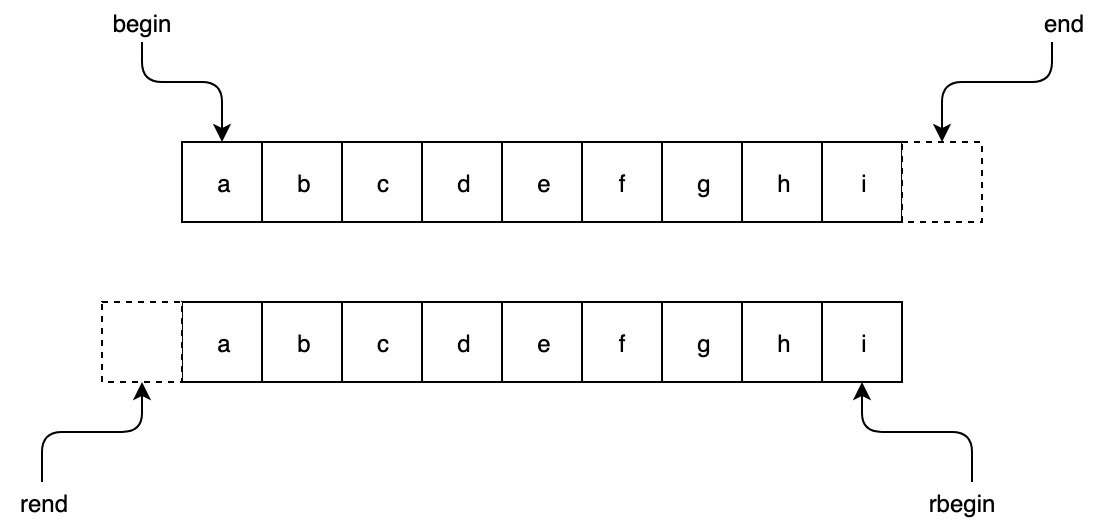
\includegraphics[align=c,width=8cm,keepaspectratio]{images/iterator_range.png}

\begin{lstlisting}[basicstyle=\ttfamily\srcbigsize]
std::begin()
std::end()
std::cbegin()
std::cend()

std::rbegin()
std::rend()
std::crbegin()
std::crend()
\end{lstlisting}
\end{center}

\end{frame}

\begin{frame}[fragile]{Некоторые адаптеры итераторов}

\begin{lstlisting}
RIt std::make_reverse_iterator(It it);

It std::front_inserter(Container & c);

It std::back_inserter(Container & c);

It std::inserter(Container & c, It it);
\end{lstlisting}

\end{frame}

\begin{frame}[fragile]{Примеры}

\begin{lstlisting}
std::vector<int> v {1, 2, 3, 4, 5};
std::deque<double> d;
auto it = std::front_inserter(d);
for (auto i : v) {
    *it++ = i;
}
std::copy(d.begin(), d.end(),
    std::ostream_iterator<double>(std::cout, ", "));
\end{lstlisting}

\begin{cmdlinelarge}
5, 4, 3, 2, 1,
\end{cmdlinelarge}

\end{frame}

%-------------------------------------------------

\section{Некоторые алгоритмы}

\begin{frame}[fragile]{Алгоритмы стандартной библиотеки}

Алгоритм -- некоторая функция, принимающая пару итераторов, задающих начало и конец последовательности и, возможно, другие аргументы.

Оперирует элементами последовательности.

\vspace{2em}

\begin{lstlisting}
std::vector<int> v { 4, 5, 3, 1, 2 };
std::sort(v.begin(), v.end() - 1);
std::copy(v.begin(), v.end(),
    std::ostream_iterator<int>(std::cout, ", "));
\end{lstlisting}

\begin{cmdlinelarge}
1, 3, 4, 5, 2,
\end{cmdlinelarge}

\end{frame}

\begin{frame}{Типы алгоритмов}

\begin{itemize}
  \item Не модифицирующие (\lstinline{any_of, for_each, count, find}) \vspace{1em}
  \item Разбивающие (\lstinline{partition}) \vspace{1em}
  \item Сортирующие (\lstinline{sort, nth_element}) \vspace{1em}
  \item Общие модифицирующие (\lstinline{copy, transform, remove, unique}) \vspace{1em}
  \item Операции над сортированными последовательностями (\lstinline{binary_search, merge, set_intersection}) \vspace{1em}
  \item И другие...
\end{itemize}

\end{frame}

\begin{frame}[fragile]{Пример модифицирующего алгоритма}

\begin{lstlisting}
std::vector<int> v { 2, 9, 10, 7, 5, 1, 3, 4, 8, 6 };

v.erase(std::remove_if(v.begin(), v.end(),
                       [] (const auto x) { return x < 5; }),
        v.end());
        
std::copy(v.begin(), v.end(),
        std::ostream_iterator<int>(std::cout, ", "));
\end{lstlisting}

\begin{cmdlinelarge}
9, 10, 7, 5, 8, 6,
\end{cmdlinelarge}

\end{frame}

\end{document}
